\section{System Design}

In this chapter, we describe the overall design in details of our disaster monitoring backend system.
Firstly, we proposed our system architecture of this disaster monitoring;
Then we specified and justify our main system components such as databases design, 
Player Task Generator, Player Rating Model as well as Disaster Evaluation Model.

With these components, model and databases, the disaster monitoring system is able to handling
common problems in HC system, such as cold start, malicious detection etc. It is also expandable,
portable and can be easily apply to any other same image selection and tagging based
human computation system in different areas.

\subsection{System Architectures}

  \begin{figure}[htp]
  \centering
  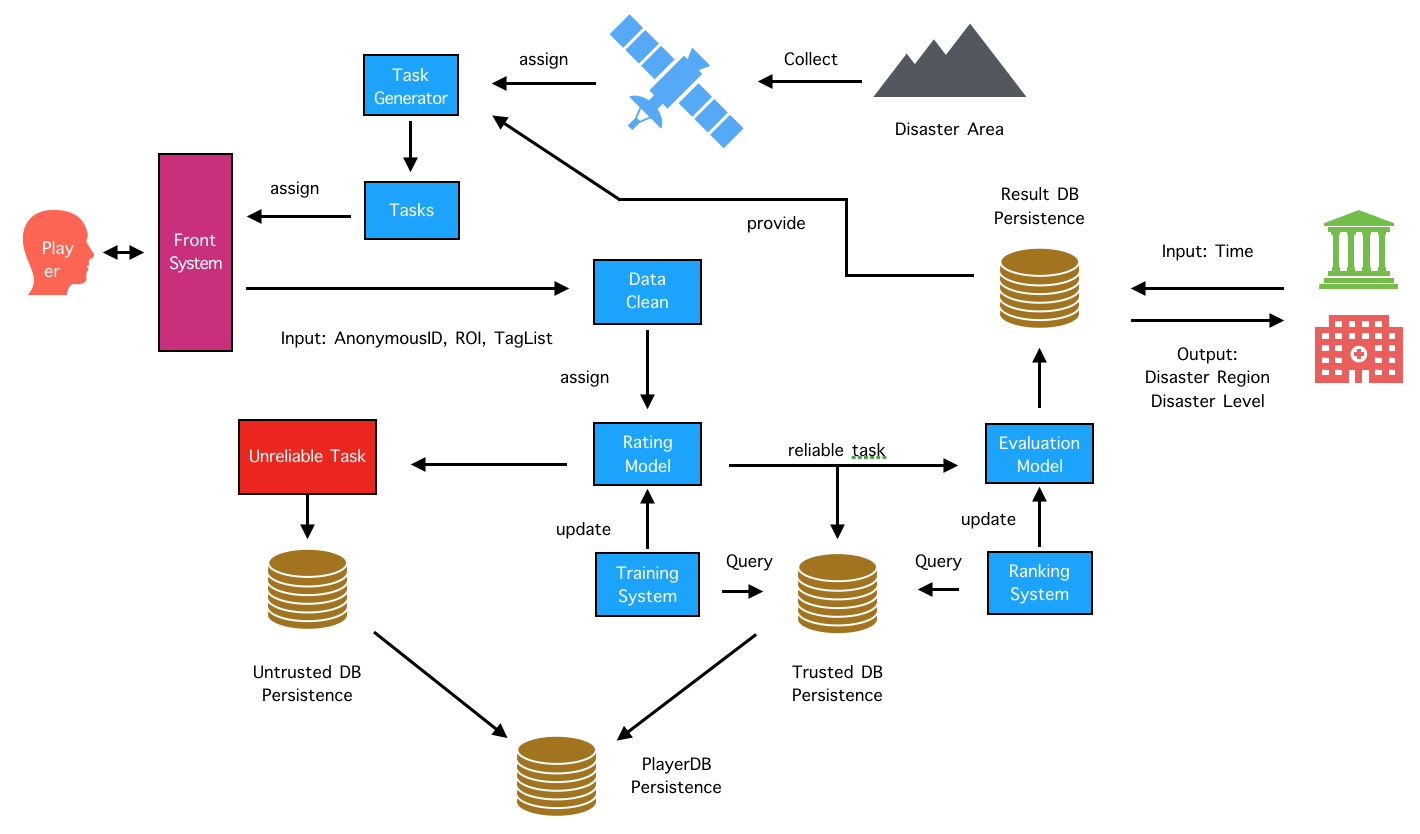
\includegraphics[width=\textwidth]{figures/system2}
  \caption{System Design Overview}
  \label{fig:arch}
  \end{figure}

  The system contains two different type of databases. The first databases \textbf{PlayerDB}
  combines with \textbf{TrustedDB} and \textbf{UntrustedDB} where
  presistent the player inputs whether the overall result is reliable or not. 
  We designed a task generator that combines 
  trusted results and seperate new satellite area images assign to upcomming players. 
  A reliable player shall pass the system \textbf{Player Rating Model}. 
  Once the task result from new player is reliable, then the system will
  reuse the player input into our \textbf{Disaster Evalutation Model} and presistent it in the second
  database \textbf{ResultDB}. Stakeholder make querys to this monitoring database. 
  Figure \ref{fig:arch} illustrate the overall disaster system design.

\subsection{System Components}

\subsubsection{Database Fields}

  For the convinience of model establishment, we describe the system database PlayerDB 
  fields as well as the fields of database ResultDB in listing \ref{lst:playerdb}
  and \ref{lst:resultdb}.

  In this disaster monitoring system, our participant do not need to register an account,
  and the system shall assign a anonymous\_id for each player, this function significantly 
  accelerate player to particpate to this game. Thus, the PlayerDB stores the anonymous\_id
  to detect the same players if they participate next time. The player will accomplish different
  game tasks, each task result shall stores in the tasks filed.

  In the ResultDB, an area ID is unique, and assigned by our system, the disaster\_level field
  represents the level of this area. Each area shall be evaluated by our player, and the evaluation
  history stores in history field.


\noindent\begin{minipage}{.45\textwidth}
\begin{lstlisting}[
    caption={Player Database Fields},
    label={lst:playerdb}
]
[
 {
  "anonymous_id": number,
  "reliable": boolean,
  "trust_value": number
  "tasks": [
   {
    "image": image_path,
    "at": time, 
    "ROI": [
     {
      "latitude": number,
      "longitude": number,
      "tags": [tag1, tag2, ...]
     }, ...
    ]
   }
  ]
 }, ...
]
\end{lstlisting}
\end{minipage}\hfill
\begin{minipage}{.45\textwidth}
\begin{lstlisting}[
  caption={Results Database Fields},
  label={lst:resultdb}
]
[
 {
  "area_id": number,
  "disaster_level": number,
  "history": [
   {
    "at": time,
    "image": image_path,
    "ROI": [
     {
      "latitude": number,
      "longitude": number,
      "tags": [tag1, tag2, ...]
    }
   ]
  }, 
  ...
 ]
}, ...
]
\end{lstlisting}
\end{minipage}


  To explain other fileds, we describe few basic definition for the system model.

  \begin{definition}
  \label{def:roi}
  The \textbf{Region of Interests (ROI)} $ROI_i$ is a player selected area of player $i$.
  \end{definition}

  \begin{definition}
  \label{def:tagv}
  The \textbf{tags vector} $T_i$ of player $i$ is indicated by a vector where the components represent by the count of all tags:
  \[
    T_i = (|\text{tag}_1|, |\text{tag}_2|, ..., |\text{tag}_n|)
  \]
  where 
  \begin{itemize}
  \item $n$ is the number of current exist tags;
  \item $|\text{tag}_n|$ is the occurrance of $\text{tag}_n$.
  \end{itemize}
  \end{definition}
  For instance, there are 5 different tags $\text{tag}_1, \text{tag}_2, \text{tag}_3, \text{tag}_4, \text{tag}_5$ exist in the current system,
  player $i$ generates tags list $\{\text{tag}_1, \text{tag}_2, \text{tag}_3\}$, player $j$ generates tag list
  $\{\text{tag}_4, \text{tag}_4, \text{tag}_5\}$. Then $T_i$ of player $i$ is $(1, 1, 1, 0, 0)$ and $T_j$ of player $j$ is $(0, 0, 0, 2, 5)$.

  \begin{definition}
  \label{def:weightv}
  The \textbf{weight vector} $v = (p(\text{tag}_1), p(\text{tag}_2), ..., p(\text{tag}_n))$ \textbf{of all tags} 
  can be calculated by the following equation \ref{eq:ptag}:
  \begin{equation}
  \label{eq:ptag}
  p(\text{tag}_i) = \frac{|\text{tag}_i|}{\sum_{j=1}^{n}{|\text{tag}_j|}}
  \end{equation}
  where
  \begin{itemize}
  \item $n$ is the number of current exist tags;
  \item $|\text{tag}_i|$ is the occurrance of $\text{tag}_i$.
  \end{itemize}
  \end{definition}

\subsubsection{Player Task Generator}

  The \textbf{Player Task Generator (PTG)} combines images from satellite and ResultDB. 
  In the first step, as we discussed before, to solve the imformation leakage problem,
  PTG shall split a monitoring region into $m\times n$ small pieces of images, and also assign a 
  unique \textbf{areaID} for each pieces, i.e. $(\text{areaID}, \text{time})$ 
  specifice a unique image for user tasks. 

  The second generate step is to retrieve tagged images from \textbf{ResultDB}. Then combine
  all images as a user task assign to a new upcomming player. Each user task contains 
  half of untagged images and half of tagged images.

  In short, The Data Model (only ouput here) for PTG is:
  $\{(\text{areaID}_1, \text{time}_1), ..., (\text{areaID}_n, \text{time}_n)\}$
  with $\text{areaID}_1$ to $\text{areaID}_{\floor{n}}$ are from satellite and 
  $\text{areaID}_{\floor{n}+1}$ to $\text{areaID}_{n}$ are from \textbf{ResultDB}.

\subsubsection{Player Rating Model}

  This subsection describes the Player Rating Model inside our Disaster Monitroing system.
  PageRank was first proposed by Lary Page \cite{page1999pagerank} and applied to social analysis in \cite{bonacich2001eigenvector}. 
  It is commonly used for expressing the stability of physical systems and the relative importance, 
  so-called centralities, of the nodes of a network. We transfer the basic idea of centralities 
  and use eigenvalue as a \textbf{Trust Value (TV)} for each players to distinguish manicious players.

  Considering a partial fully connected directed graph betwen players. 
  Each player is a node of the Player Rating Graph (PRG) as illustrate in figure \ref{fig:graph}.

  \begin{figure}[htp]
  \centering
  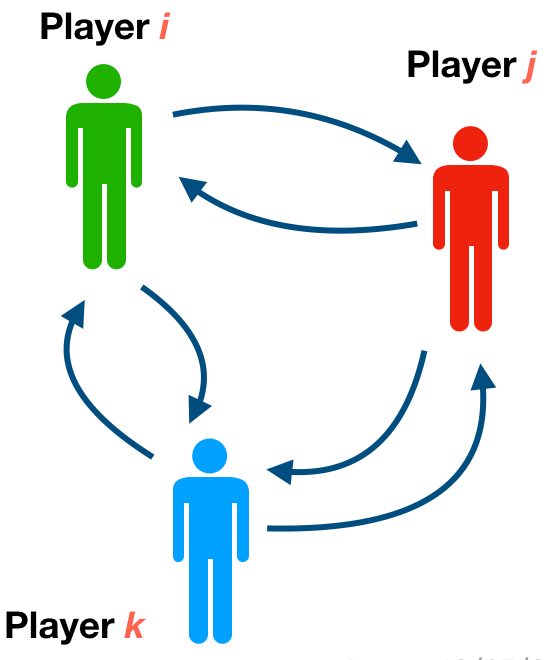
\includegraphics[width=0.3\columnwidth]{figures/graph}
  \caption{Player Rating Model}
  \label{fig:graph}
  \end{figure}
  
  To define the edge weight, according to the database feild design of a player, each player
  output ROIs for each task region of a player task, and each ROI contains a tags list, thus, 
  one can use three festures: $\text{ROI}, \text{tags}, TV$.

  \begin{definition}
  The weight from player $i$ to player $j$ can be formalized as follows formula \ref{eq:weight}:
  \begin{equation}
  \label{eq:weight}
  w_{ij} = 
  \sum_{\text{ROI}\in\text{ROIs}}{\left(
    \text{TV}_i \times
    \frac{\text{ROI}_i\cap\text{ROI}_j}{\text{ROI}_i}\times
    \left( 2-\frac{Cov(T_i, T_j; v)}
        {Cov(T_i, T_i; v)\times Cov(T_j, T_j; v)} \right)\right)
  }
  \end{equation}

  where 
  
  \begin{itemize}
    \item $TV_i$ is the trust value of player $i$;
    \item $\text{ROI}_i$ is the selected ROI from player $i$;
    \item $T_i$ is the tags vector of player $i$;
    \item $Cov(x, y; v)$ is the weighted covariance of $x$ and $y$ via $v$;
    \item $v$ is the weight vector of all tags.
  \end{itemize}
  \end{definition}

  The first part of the definition $\sum_{\text{ROI}\in\text{ROIs}}$ summarized all possible 
  ROI between player $i$ and player $j$. The theioretically item of this formular is the number
  of ROI from player $i$ multiply the number of ROI from player $j$. Nevertheless, it can be
  significantlly decreased in this particular scienario. Considering player i and player j 
  with two ROIs as illustrate in figure \ref{fig:performance}.

  \begin{figure}[htp]
  \centering
  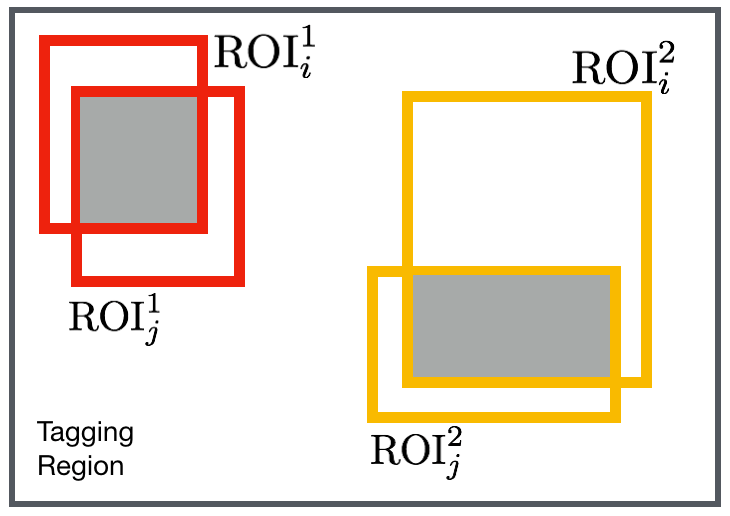
\includegraphics[width=0.5\columnwidth]{figures/performance}
  \caption{Two players with two ROIs}
  \label{fig:performance}
  \end{figure}

  One can expand equation \ref{eq:weight} as follows formula \ref{eq:expand}:

  \begin{multline}
  \label{eq:expand}
  w_{ij} = \text{TV}_i \times \left(2-\frac{Cov(T_i, T_j; v)}{Cov(T_i, T_i; v)\times Cov(T_j, T_j; v)}\right) \times \\
    \left( \frac{\text{ROI}_i^1\cap\text{ROI}_j^1}{\text{ROI}_i^1}           
    + \frac{\text{ROI}_i^1\cap\text{ROI}_j^2}{\text{ROI}_i^1}           
    + \frac{\text{ROI}_i^2\cap\text{ROI}_j^1}{\text{ROI}_i^2}           
    + \frac{\text{ROI}_i^2\cap\text{ROI}_j^1}{\text{ROI}_i^2} \right)
  \end{multline}

  Fortunately, the second and the third part of the expation are equal to zero.

  We call the second part $\text{TV}_i \times \frac{\text{ROI}_i\cap\text{ROI}_j}{\text{ROI}_i}$ 
  of formula \ref{eq:weight} as \textbf{Matching Area Ratio (MAR)}. 
  It was inspired by a common computer vision criteria,
  the so called Intersection over Union (IoU), also called Jaccard Index in mathematics\cite{real1996probabilistic},
  which is the standard performance measure that is commonly used for the object category segmentation problem.
  Nevertheless, MAR is not equal to the IoU of ROIs of player $i$  and player $j$ since
  it only use the ROI of player $i$ as denominator instead of the union of ROIs of player $i$ and player $j$,
  which leads the differnce between MAR and IoU. There are two reason to use MAR instead of IoU:
  Firstly, IoU as weight of graph causes the directed graph to an undirected graph due to the IoU of player $i$ to $j$
  is as same as the IoU of player $j$ to $i$; Furthermore, player $i$ as the evaluator from $i$ to $j$ 
  should be the performance base.

  The third part $\frac{Cov(T_i, T_j; v)}{Cov(T_i, T_i; v)\times Cov(T_j, T_j; v)}$
  of formula \ref{eq:weight} is applied by Weighted Pearson Correlation Coefficient.
  
  To calculate the eigenvalue of the ajacency matrix of PRG, one can use the normalized ajacency matrix 
  through the following formula \ref{eq:normalize}:
  \begin{equation}
  \label{eq:normalize}
  A = (a_{ij}) = (\frac{w_{ij}}{\sum_{j}{w_{ij}}})\\
  \end{equation}

  \begin{theorem}
  Matrix $A$ is irreducible, real, non-negative, column-stochastic, and diagonal element being positive.
  \end{theorem}

  \begin{proof}
  \textbf{Irreducibility}: $A$ is normalized through an ajacency matrix of a strong connected player
  rating graph, which proves $A$ is irreducible.

  \textbf{Real elements}: Trivial.
  
  \textbf{Non-negative elements}: We only need to prove $\text{TV}_i$, 
    $\frac{\text{ROI}_i\cap\text{ROI}_j}{\text{ROI}_i}$ and 
    $2-\frac{Cov(T_i, T_j; v)}{Cov(T_i, T_i; v)\times Cov(T_j, T_j; v)}$ are non-negative 
    respectively. $\text{TV}_i$ is the eigenvalues of normalized graph ajacency matrix, 
    thus the codomain of $\text{TV}_i$ lies $(0, 1\rbrack$; For MAR, its range is obviously from 0 to 1,
    which lies $\lbrack 0, 1 \rbrack$; For $2-\frac{Cov(T_i, T_j; v)}{Cov(T_i, T_i; v)\times Cov(T_j, T_j; v)}$,
    the Pearson Correlation lies on $[-1, 1]$, then this part lies on $[1, 3]$.
    Three parts are non-negative.
  
  \textbf{Positive diagonal elements}: The diagonal elements can be formalized by follows:

  \[
  w_{ii} = 
  \sum_{\text{ROI}\in\text{ROIs}}{\left(
    \text{TV}_i \times
    \frac{\text{ROI}_i\cap\text{ROI}_i}{\text{ROI}_i}
    \left( 2-\frac{Cov(T_i, T_i; v)}
        {Cov(T_i, T_i; v)\times Cov(T_i, T_i; v)} \right)\right)
  } = \sum_{\text{ROI}\in\text{ROIs}}{\text{TV}_i} > 0
  \]
  
  \textbf{Column stochastic}: according to the definition of matrix $A$, the sum of the column
  elements is:
  \[
    \sum_{i}{\frac{w_{ij}}{\sum_{j}{w_{ij}}}} 
    = \frac{\sum_{i}{w_{ij}}}{\sum_{j}{w_{ij}}} = 1
  \]
  \end{proof}

  We has proved the existence and uniqueness of eigenvalues of normalized PRG ajacency matrix, 
  one can use the corresponding eigenvalues to represent the trust value of players. Thus, we have:

  \begin{definition}
  A \textbf{Trust Value} $TV_i$ of player $i$ represents by the $i$-th eigenvalue of normalized PRG ajacency matrix $A$.
  \end{definition}

  This definition can represents the rating score from $i$ to $j$. With the trust value of players,
  we propose our classification algorithm:

  \begin{algorithm}[H]
  \SetAlgoLined
  \SetKwInOut{Input}{input}\SetKwInOut{Output}{output}
  \Input{anonymous IDs, TVs}
  \Output{(anonymous\_id, isReliable)}
  Calculate $TV_{new}$ as the trust value of player $new$ \;
  \eIf{$TV_{new} \geq \frac{1}{|\text{players}|}\sum_{i\in \text{players}}{TV_{i}}$}{
    return $(\text{anonymous\_id}, \text{true})$
  }{
    return $(\text{anonymous\_id}, \text{false})$
  }
  \caption{Player Classification Algorithm}
  \end{algorithm}

  In this algorithm, the criterion of classify new players performs the action that 
  the trust value of new player should not less than the mean value of overall trust value of players, 
  which means the tagging performance of new player should not worth than result performance of former players.
  
  Terefore in short, the input and output Data Model of PRM are as follows. For input:\\
  $(\text{anonymous\_id}, \text{area\_id}, \text{time}, \text{ROIs}, \text{tags})$; 
  For model output: 
  $(\text{anonymous\_id}, \text{TV})$.

  \subsubsection{Disaster Evaluation Model}
  \label{chapter:dem}

  For an area at time $t$, we address the \textbf{Disaster Evaluation Model (DEM)} 
  via disaster level definition as follows:

  \begin{definition}
  \label{def:dl}
  The \textbf{Disaster Level (DL)} of a monitor region is calculated by each area components:
  \[
    DL = \sum_{\text{area}\in\text{region}}{DL_{\text{area}}}
  \]
  where $DL_{\text{area}}$ is calculated by its corresponding tag vector:
  \[
    DL_{\text{area}} = \sum_{i=1}^{n}{v_i \times |\text{tag}_i|}
  \]
  with $n$ is the number of current exist tags, and $|\text{tag}_i|$ is the occurrance of $\text{tag}_i$
  in the corresponding area.
  \end{definition}

  System like ESP\cite{von2004labeling}, ARTigo\cite{wieser2013artigo} has proved that 
  human inputs are valuable and useful.

  Note that sometimes player carries new tags for our system, we also address a solution 
  for this issue via the following steps:

  \begin{itemize}
  \item When a player carries predefined tags: Trivial;
  \item When a player carries new tags: Directly drop, it is an unreliable result;
  \item When a player carries predefined tags and also new tags: calculate the trust value without new tags;
   merge and update all weight vector $v$ via formula \ref{eq:weight} if the player is reliable, 
   otherwise drop and mark the result is unreliable.
  \end{itemize}

  With this definition \ref{def:dl}, we can calculate the disaster level for a monitoring region.
  To sum up, the input and the output Data Model of DEM addresse as follows. For input:
  $(\text{time})$, $(\text{area\_id})$ or $(\text{area\_id}, \text{time})$; For output:
  $(\text{area\_id}, \text{time}, \text{disaster\_level})$.

\subsection{Model Initialization and System Cold Start}

  A cold start of such a system is a common problem in human computation system that 
  is avoided by hiring people to play or learn as long as 
  the number of users or the quantity of data is insufficient.
  In our system, we have two different cold start problem.

  The first cold start problem appears in the PTG. To initialize the whole system, we need
  address a initial trusted group for PTG, they shall tagging ennough initial trusted result
  for PTG and then assign to new upcomming players. When a new player is reliable,
  then the result of this player will become reliable. Meanwhile, the trusted group and avaliable 
  dataset become larger with this step repeatedly, as shown in figure \ref{fig:cold}.

  \begin{figure}[htp]
  \centering
  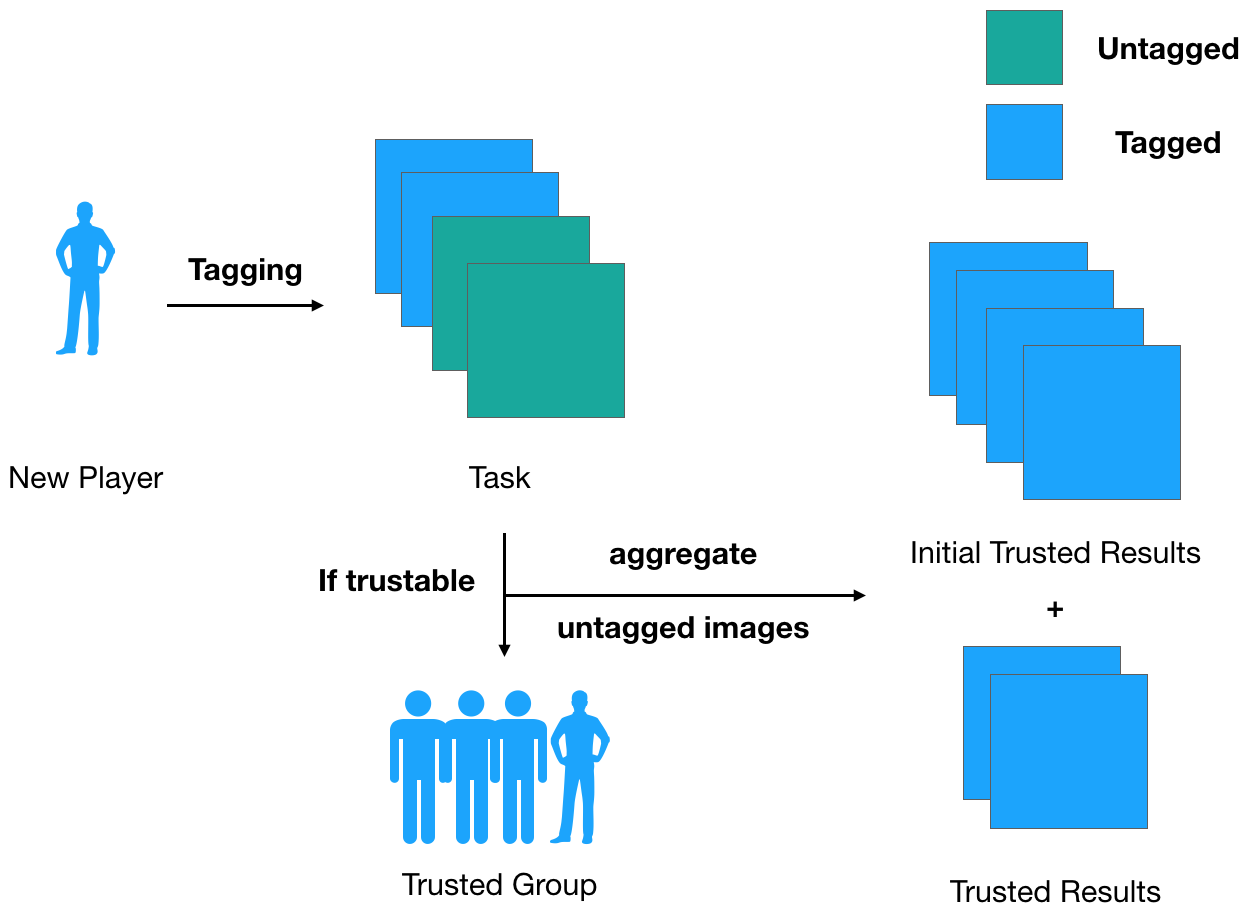
\includegraphics[width=0.5\columnwidth]{figures/coldstart}
  \caption{Cold Start of PTG}
  \label{fig:cold}
  \end{figure}

  The second cold start problem appears in PRM. According to the definition \ref{def:weight} of PRG, the weight
  of PRG was defined by the trust value of all players. Nevertheless the initial trusted group has
  no trust value. Thus we need a initial value for $TV$. Note that TV\_i is in between of 0 and 1, thus:

  \[
  TV_{i}^{\text{init}} = \frac{1}{|\text{players}^{\text{init}}|}
  \]

  with $|\text{players}^{init}|$ is the number of initial trusted group. 